\section{Vision Transformers}

\begin{frame}{Processing Text}
    \begin{itemize}
        \item \textbf{Token Embeddings}: The input text is broken down into individual tokens. 
	\item \textbf{Word Embeddings}: Each token is converted into a fixed-length vector representation.
	\item \textbf{Self-Attention on Tokens}: The transformer's self-attention mechanism is applied to these word embeddings. 
    \end{itemize}
\end{frame}

\begin{frame}{Processing Images}
    \begin{itemize}
        \item \textbf{Patch Embeddings}: ViT splits an image into fixed-size patches (e.g., $16\times16$ pixels). Each patch is treated like a token in NLP, much like words in a sentence.
	\item \textbf{Linear Embedding}: Each patch is flattened into a 1D vector and then linearly projected to a fixed-length embedding.
	\item \textbf{Self-Attention on Patches}: The Transformer’s self-attention mechanism is then applied to these patch embeddings, allowing the model to learn relationships between patches.
    \end{itemize}
\end{frame}

\begin{frame}{ViT Overview}
    \begin{figure}
        \centering
        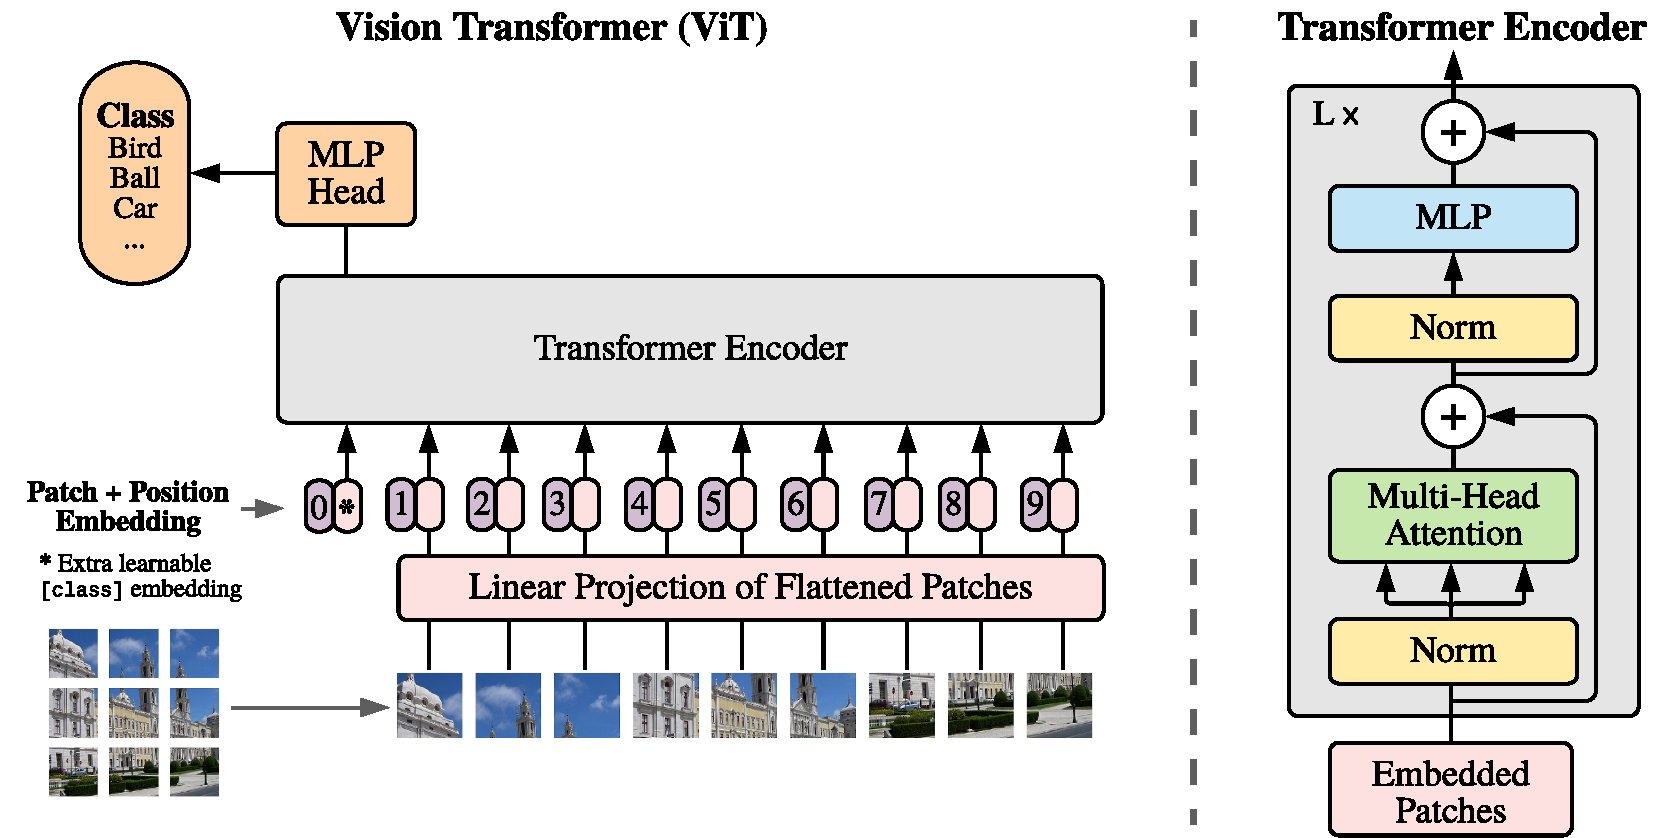
\includegraphics[width=0.95\linewidth]{pic/model_scheme}
        % \caption{We split an image into fixed-size patches, linearly embed each of them, add position embeddings, and feed the resulting sequence of vectors to a standard Transformer encoder. In order to perform classification, we use the standard approach of adding an extra learnable “classification token” to the sequence.}
        \label{fig:vit-figure}
    \end{figure}
\end{frame}



\begin{frame}{Patch Sizes}
    \begin{itemize}
        \item Patch size determines the granularity of the image representation.
        \item Smaller patches capture finer details but increase computational cost.
        \item The self-attention mechanism has $\mathcal{O}(N^2)$ complexity due to pairwise interactions between $N$ patches. 
        \item Larger patches reduce computational complexity but might miss finer details.
        \item In practice: 
            \begin{itemize}
                \item take 224x224 input image,
                \item divide it into a 16x16 grid of 14x14 pixel patches (or 14x14 grid of 16x16 patches)
            \end{itemize} 
        \item \textbf{An Image is Worth 16x16 Words!}
    \end{itemize}
\end{frame}


\begin{frame}{Positional Embeddings}
    \begin{itemize}
        \item We need to inject spatial information into the model to ensure the model understands the order of image patches.
        \item There are several options: 
        \begin{itemize}
            \item Providing no positional information: \textit{bag of patches}
            \item 1-dimensional positional embedding: sequence of patches in the raster order
            \item 2-dimensional positional embedding: concatenate embedding of different axes
            \item Relative positional embeddings: relative distance instead of absolute position
        \end{itemize}
        \item In practice 1-dimensional positional embedding work best.
    \end{itemize}
\end{frame}



\begin{frame}{Combining Patches and Embeddings}
    \begin{enumerate}
        \item \textbf{Divide Image into Patches}
        \begin{itemize}
            \item Image of size \( H \times W \) divided into patches of size \( P \times P \).
            \item Number of patches: \( N = \frac{H \times W}{P \times P} \).
        \end{itemize}
        \item \textbf{Flatten and Project Patches}
            \[
            \text{patch\_embedding}_i = \text{Linear}(\text{flatten}(x_i))
            \]
        \item \textbf{Add Positional Embeddings}
           \[
            \text{combined\_embedding}_i = \text{patch\_embedding}_i + PE_i
            \]
        \item \textbf{Form Input Sequence}
            \[
            \text{Input} = [\text{CLS}; \text{combined\_embedding}_1; \ldots; \text{combined\_embedding}_N]
            \]
    \end{enumerate}
\end{frame}


\begin{frame}{Transformer Encoder}
    \begin{itemize}
        \item Now that we have an \textbf{Input Sequence}, we can use a simple Transformer Encoder.
        \item A Transformer encoder consists of:
        \begin{itemize}
            \item  Multi-Head Attention: Learns relationships between all tokens (image patches) in the sequence.
        	\item Feedforward Network: Processes each token independently in a higher-dimensional space.
	        \item Residual Connections \& Layer Normalization: Helps with optimization.
        \end{itemize}
        \item Finally we can pass the output of the encoders to an MLP classifier head in order to predict the correct class.
    \end{itemize}
\end{frame}

\begin{frame}{Batch Normalization}
    \begin{columns}
        \begin{column}{0.65\linewidth}
        \begin{itemize}
            \item Normalizes inputs across the mini-batch.
            \[
            \hat{x}_{ij} = \frac{x_{ij} - \mu_{j}}{\sqrt{\sigma^2_{j} + \epsilon}}
            \]
            where \( \mu_{j} \) and \( \sigma^2_{j} \) are the mean and variance of the \( j \)-th feature in the mini-batch.
            \item Appropriate for CNNs.
            \item Requires large batch sizes.
            \item Improves generalization via regularization.
        \end{itemize}
        \end{column} 
        \begin{column}{0.4\linewidth} 
        \begin{figure}
            \centering
            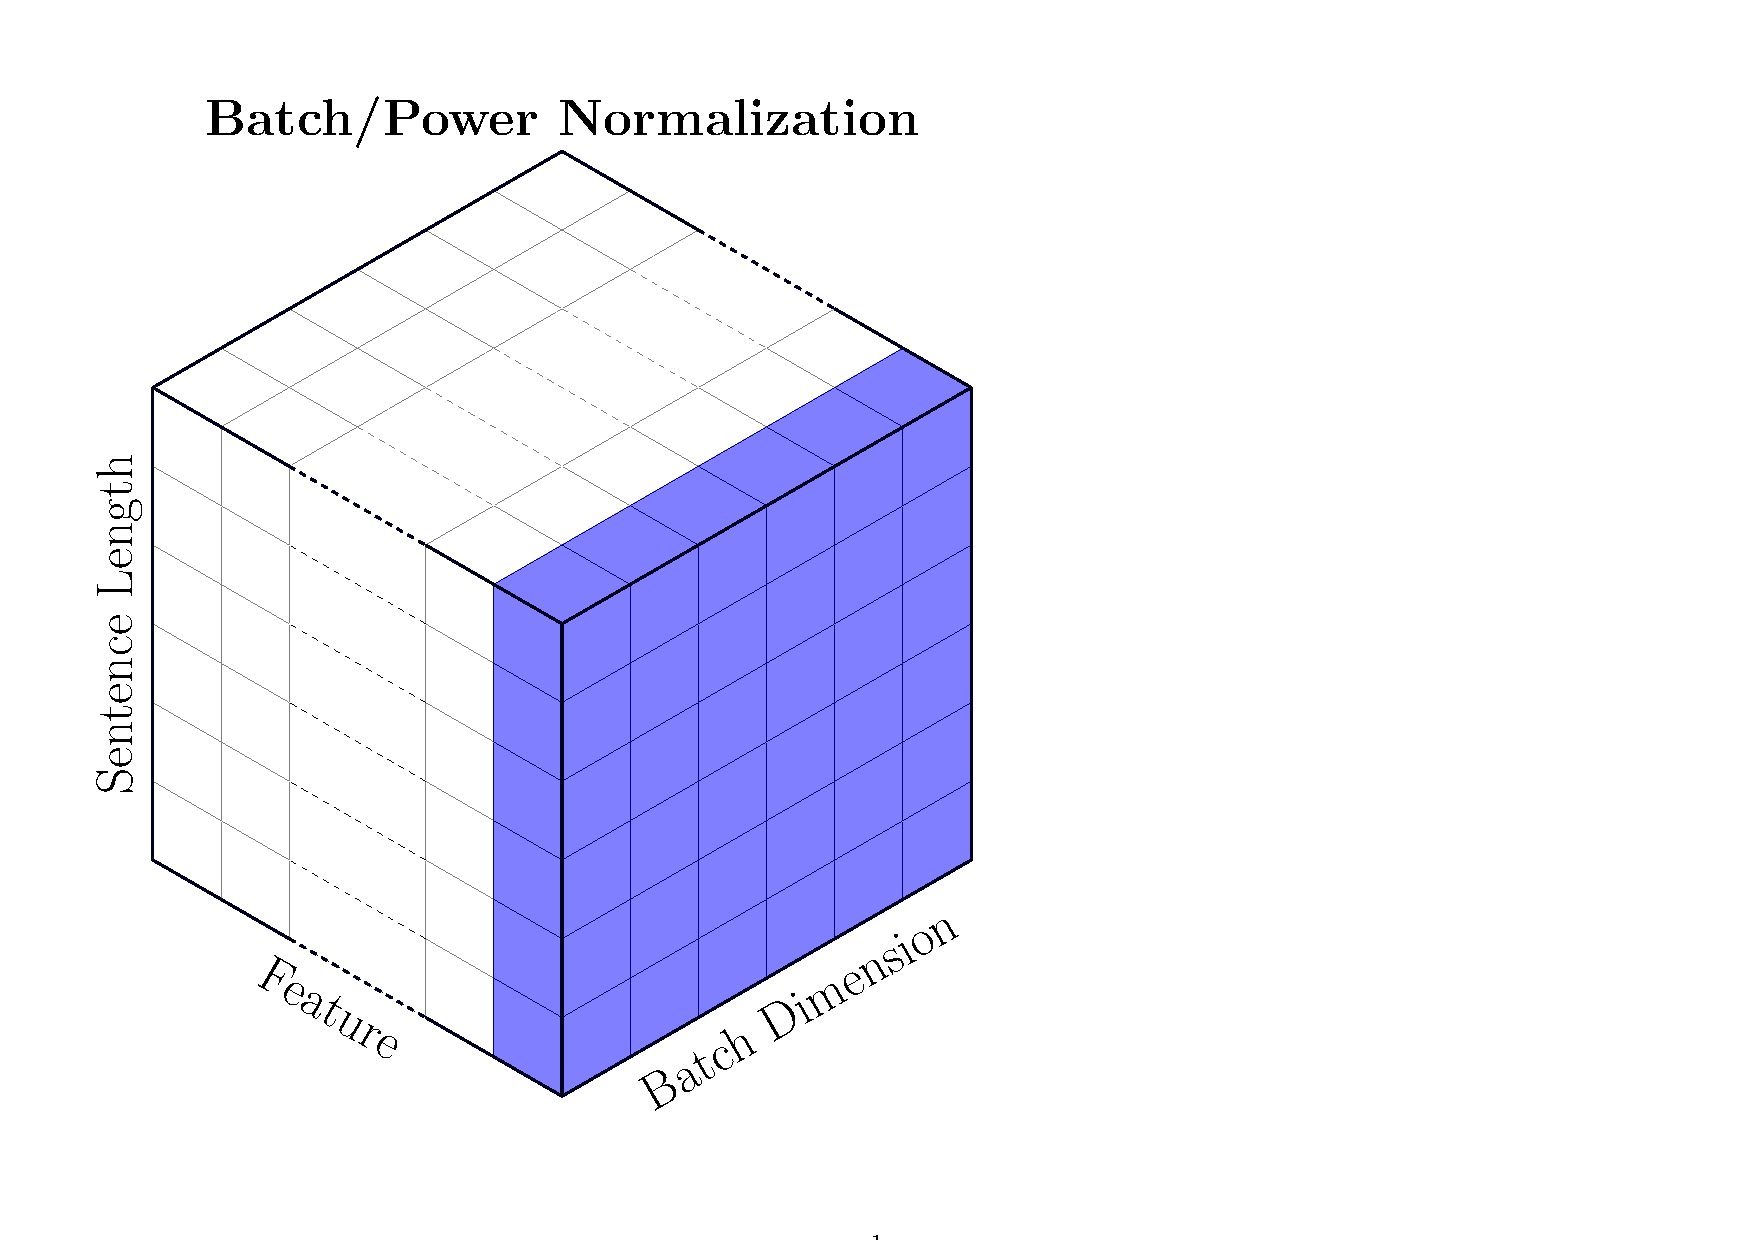
\includegraphics[width=1.5\linewidth]{pic/PN_vis.pdf}
            \label{fig:bn}
        \end{figure}
        \end{column}
    \end{columns}
\end{frame}

\begin{frame}{Layer Normalization}
    \begin{columns}
        \begin{column}{0.65\linewidth}
        \begin{itemize}
            \item Normalizes inputs across the features in a single training example.
            \[
            \hat{x}_{ij} = \frac{x_{ij} - \mu_{i}}{\sqrt{\sigma^2_{i} + \epsilon}}
            \]
            where \( \mu_{i} \) and \( \sigma^2_{i} \) are the mean and variance of the \( i \)-th training example.
            \item Appropriate for Transformers, RNNs, or NLP tasks.
            \item Works with small or dynamic batch sizes.
            \item Provides batch-independent normalization for flexibility.
        \end{itemize}
        \end{column} 
        \begin{column}{0.4\linewidth}
        \begin{figure}
            \centering
            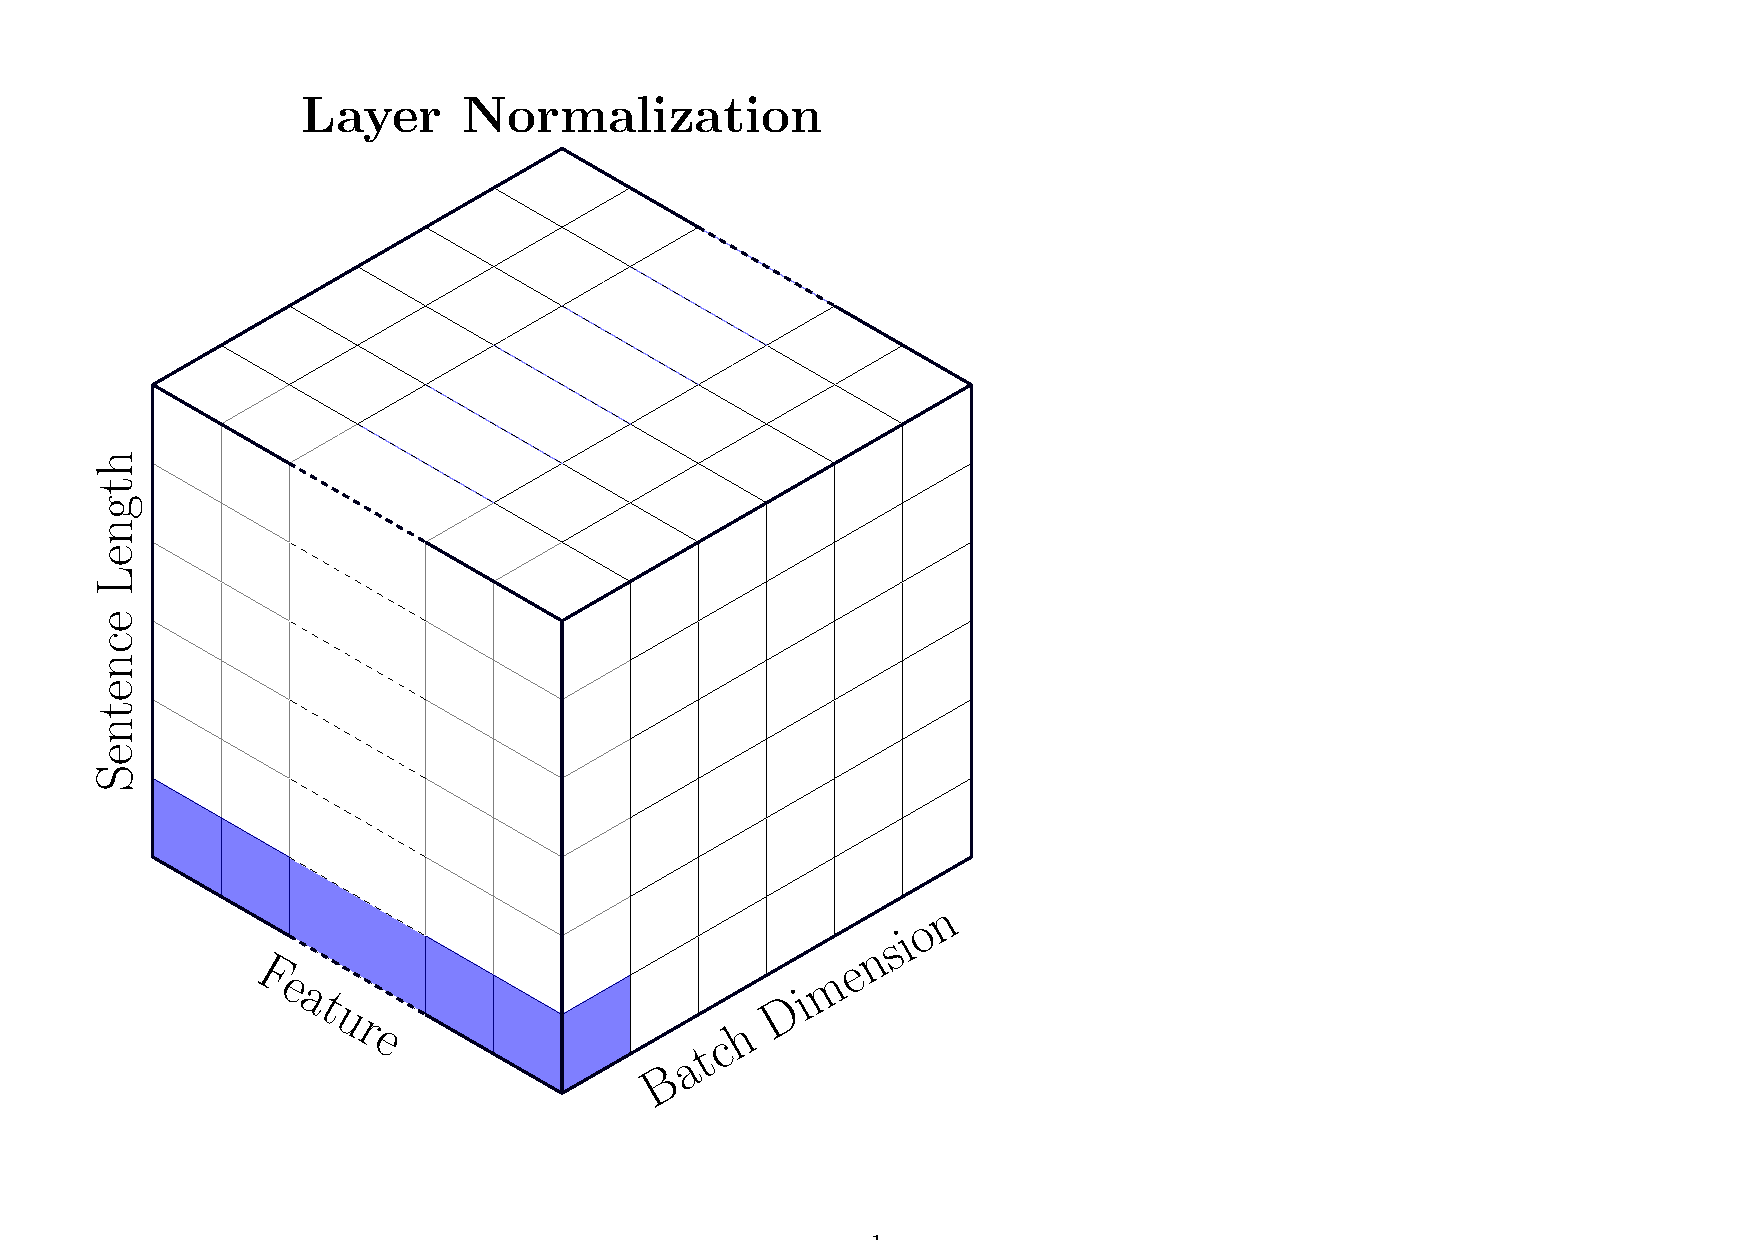
\includegraphics[width=1.5\linewidth]{pic/LN_vis.pdf}
            \label{fig:ln}
        \end{figure}
        \end{column}
    \end{columns}
\end{frame}

% \begin{frame}{Choosing The Right Normalization Scheme}
%     % \begin{tabular}{|p{2cm}|p{5cm}|p{5cm}|}
%     %     \hline
%     %     \textbf{Scheme} & \textbf{Advantages} & \textbf{Disadvantages} \\ \hline
%     %     \textbf{BatchNorm} & 
%     %     \begin{itemize}
%     %         \item Reduces internal covariate shift.
%     %         \item Acts as a regularizer.
%     %         \item Speeds up training.
%     %     \end{itemize} & 
%     %     \begin{itemize}
%     %         \item Depends on batch size.
%     %         \item Inefficient for small-batch or online learning.
%     %         \item Computational overhead.
%     %     \end{itemize} \\ \hline
%     %     \textbf{LayerNorm} & 
%     %     \begin{itemize}
%     %         \item Works with small batches.
%     %         \item Invariant to batch size.
%     %         \item Simple implementation.
%     %     \end{itemize} & 
%     %     \begin{itemize}
%     %         \item Less effective in CNNs.
%     %         \item Weaker regularization.
%     %     \end{itemize} \\ \hline
%     % \end{tabular}
% \end{frame}



\begin{frame}{What Do Positional Embeddings Learn?}
    \begin{columns}
        \begin{column}{0.6\textwidth}
            \begin{itemize}
                \item The model learns to encode distance within the image in the similarity of position embeddings.
                \item This means closer patches tend to have more similar position embeddings. 
                \item Patches in the same row/column have similar embeddings.
            \end{itemize}
        \end{column}
        \begin{column}{0.4\textwidth}
            \begin{figure}
                \centering
                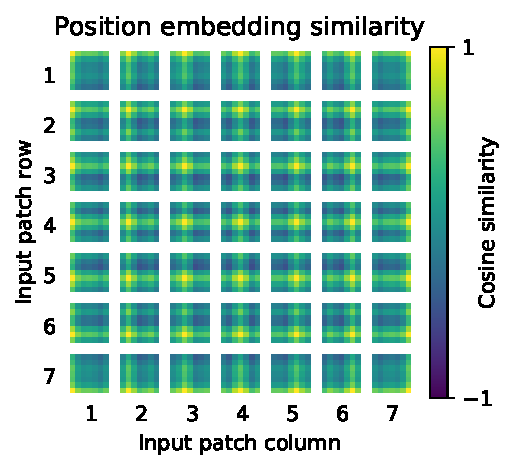
\includegraphics[width=\linewidth]{pic/20201002_position_embeddings_17085772_1.pdf}
                % \caption{Visualization of Positional Encodings}
                \label{fig:pos_encodings}
            \end{figure}
        \end{column}
    \end{columns}
\end{frame}

\begin{frame}{How Does Attention Help?}
    \begin{columns}
        \begin{column}{0.65\textwidth}
            \begin{itemize}
                \item Self-attention allows ViT to integrate information across the entire image even in the lowest layers.
                \item We can average attention weights across all heads and recursively multiply the weight matrices of all layers to mix attention across tokens through all layers.
            \end{itemize}
        \end{column}
        \begin{column}{0.35\textwidth}
            \begin{figure}
                \centering
                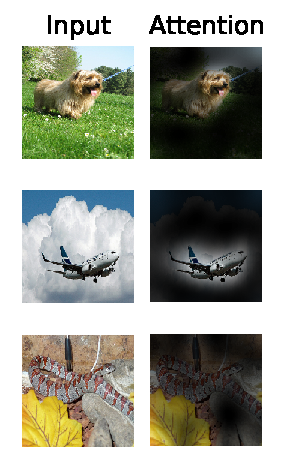
\includegraphics[width=0.8\textwidth]{pic/20201002_selected_attention_examples}
                % \caption{Representative examples of attention from the output token to the input space.}
                \label{fig:inspecting-vit}
            \end{figure}
        \end{column}
    \end{columns}
\end{frame}

